\documentclass[../../thesis.tex]{subfiles}

\newcommand{\inner}[2]{\left<#1, #2\right>}
\newcommand{\alemap}{\ensuremath{\mathcal{A}}}
\newcommand{\dt}{\ensuremath{\Delta t}}
\newcommand{\pexp}{\ensuremath{\frac{2\gamma}{\left(\gamma-1\right)}}}
\newcommand{\aleX}{\ensuremath{\mathcal{X}}}
\newcommand{\Ah}[1]{\ensuremath{\vb{#1}^{n+1}_h}}
\newcommand{\Ahn}[1]{\ensuremath{\vb{#1}^{n}_h}}

\newcommand{\rbV}{\ensuremath{\mathbb{V}}}
\newcommand{\rbVT}{\ensuremath{\rbV^T}}
\newcommand{\epspod}{\ensuremath{\varepsilon_\text{POD}}}

\begin{document}

\section{Parameter Range}
For the construction of the reduced basis we are randomly sampling the parameter space.
Hence, we need to determine an acceptable range for each parameter.

To do so, we sample a large space and visually check each of the solutions.
Visual inspection reveals that certain solutions contain wiggles when a shock wave occurs, see Figure~\ref{fig:smooth_vs_wiggled}.
Naturally, wiggles were not expected to be captured by this simple model, 
so they must be due to the fact that the shock wave is becoming thinner than the mesh size.

\begin{figure}[h]
    \centering
    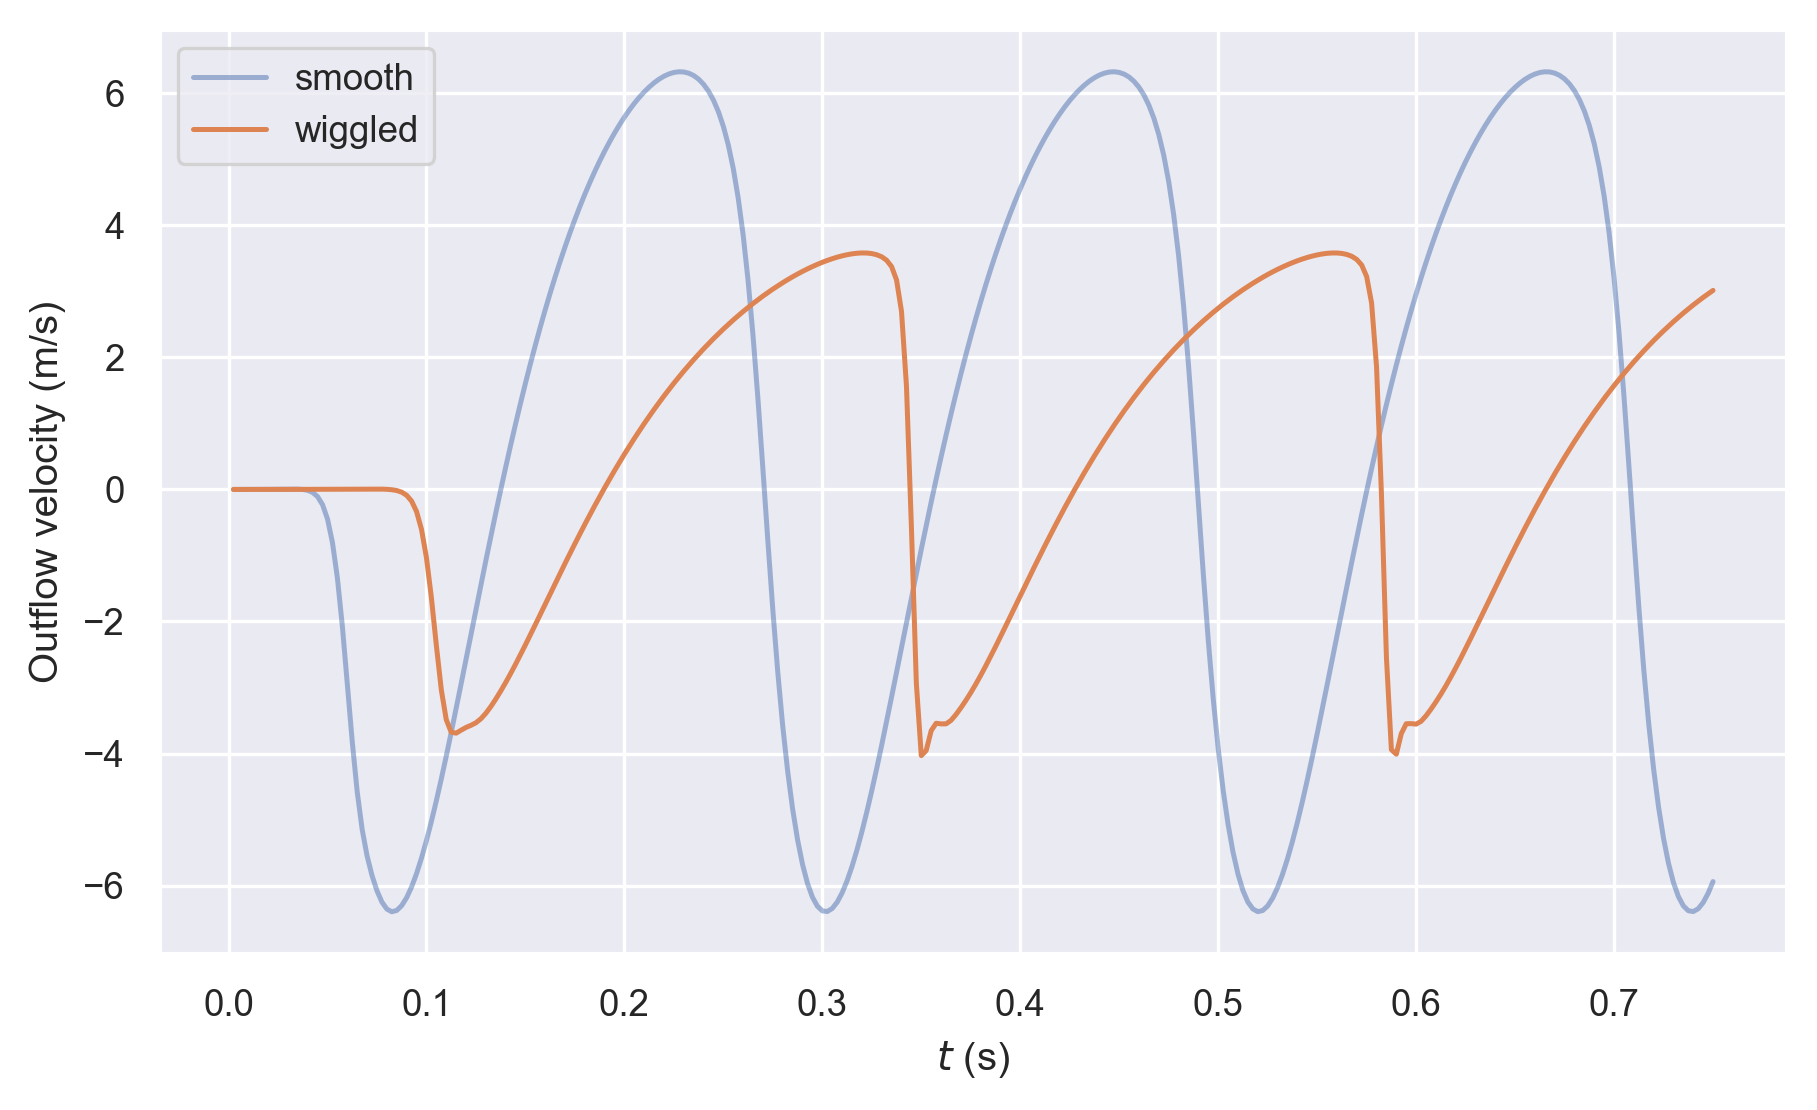
\includegraphics[width=1\columnwidth]{research_project/piston/figures/wiggles/smooth_vs_wiggled.png}
    \caption{Smooth and wiggled solutions comparison.
    Each solution has a different scale and frequency because they were obtained for different parametrizations.}
    \label{fig:smooth_vs_wiggled}
\end{figure}
To prevent these unrealistic solutions from polluting our reference solutions, we
need to determine a safety margin in the sampling range prevent using a parametrization for which wiggles will take place.


\subsection{System Forcing And Nonlinear Response}
\label{sec:fom_calibration_system_forcing}
\mytodo{State this has to do with the way we have stabilized the discretization.}
On the one hand, when we think about the equations and their response, we could hint at the fact that shock wave strength will be driven by the magnitude of the piston's velocity.
This variable, although time dependent, is scaled by the combination of the speed of sound,
piston frequency and displacement, 
namely the piston peak velocity
\begin{equation}
    u_p \sim \frac{\delta \omega L_0}{a_0}.
\end{equation}
Such peak velocity will be maximum (minimum) for maximum (minimum) values of displacement and frequency, and minimum (maximum) values for the speed of sound.

On the other hand, we need a procedure to quantify the nonlinearity of the system response.
In the absence of the nonlinear term, the equations would reduce to a linear convection model.
In such model we would expect the piston motion to be perfectly convected towards the outflow.
But due to the presence of the nonlinear term, we know this will not be the case.
Hence, we suggest and use as a nonlinearity metric $\eta$ the ratio between the time between two peaks at the ouflow and the piston,
\begin{equation}
    \eta := \frac{T}{T_0},
\end{equation}
where $T$ and $T_0$ are respectively defined as
\begin{subequations}
    \begin{align}
        T_0 &:= t^{L}_{+} - t^{L}_{-},
        \\
        T   &:= t^{\text{out}}_{+} - t^{\text{out}}_{-}.
    \end{align}
\end{subequations}
The symbols $t^{(\cdot)}_{+}$ and $t^{(\cdot)}_{-}$ denote the first positive and the second\footnote{We take the second negative peak and not the first one to remove any possible distortion due to the initial transient from rest to harmonic movement.} negative peaks in the velocity function at their respective locations.

The closer $\eta$ is to one, the more linear the response is.
As it tends to zero, the response is becoming nonlinear, 
since a shock wave is building up at the outflow;
\begin{align*}
    &\eta \sim 1 : \text{Linear response}, 
    \\
    &\eta \rightarrow 0 : \text{Nonlinear response}.
\end{align*}
In Figure~\ref{fig:wiggle_correlation} we show the response of the system for different parametrization values, alongside with the forcing $u_p$ and nonlinearity measure $\eta$. 
We have manually tagged which combinations present wiggles.
There are several observations to be made about this pair plot.

First of all, looking the raw parameters $a_0, \omega$ and $\delta$, we observe how 
none of them individually explain how nonlinear the response of the system will be.
There is certainly a trend, low values of $a_0$ and large values of $\delta$ and $\omega$ contain wiggles (as shown by the density plots). 
However, points with low values of $a_0$ belong to the set without wiggles too. 
Therefore, it must be the combination of them which explains the existence of wiggles.

When we look at the correlation between~$u_p$ and~$\eta$, we observe a linear trend between them: the higher the forcing, the stronger the nonlinearity in the response.
And clearly, beyond a threshold in the forcing, the system seems to break and most solutions contain wiggles.
This critical value~$u_M$ for the forcing seems to be in the neighborhood of~$u_M \sim 0.4$. 

With this empirical study of the system's response (and after running some tests) we choose the following ranges for our parameters:
\begin{table}[h]
    \centering
    \caption{Acceptable parameter range for random sampling. This configuration should prevent the existence of wiggles at the outflow.}
    \begin{tabular}{cccc}
    \toprule
        Variable  & Minimum & Maximum & Units 
        \\ \midrule
        $a_0$     & 18      & 25      & m/s \\
        $\omega$  & 15      & 30      & 1/s \\
        $\delta$  & 0.15    & 0.3     & [-]
        \\ \bottomrule
    \end{tabular}
\end{table}


\onecolumn
\begin{figure}[h]
    \centering
    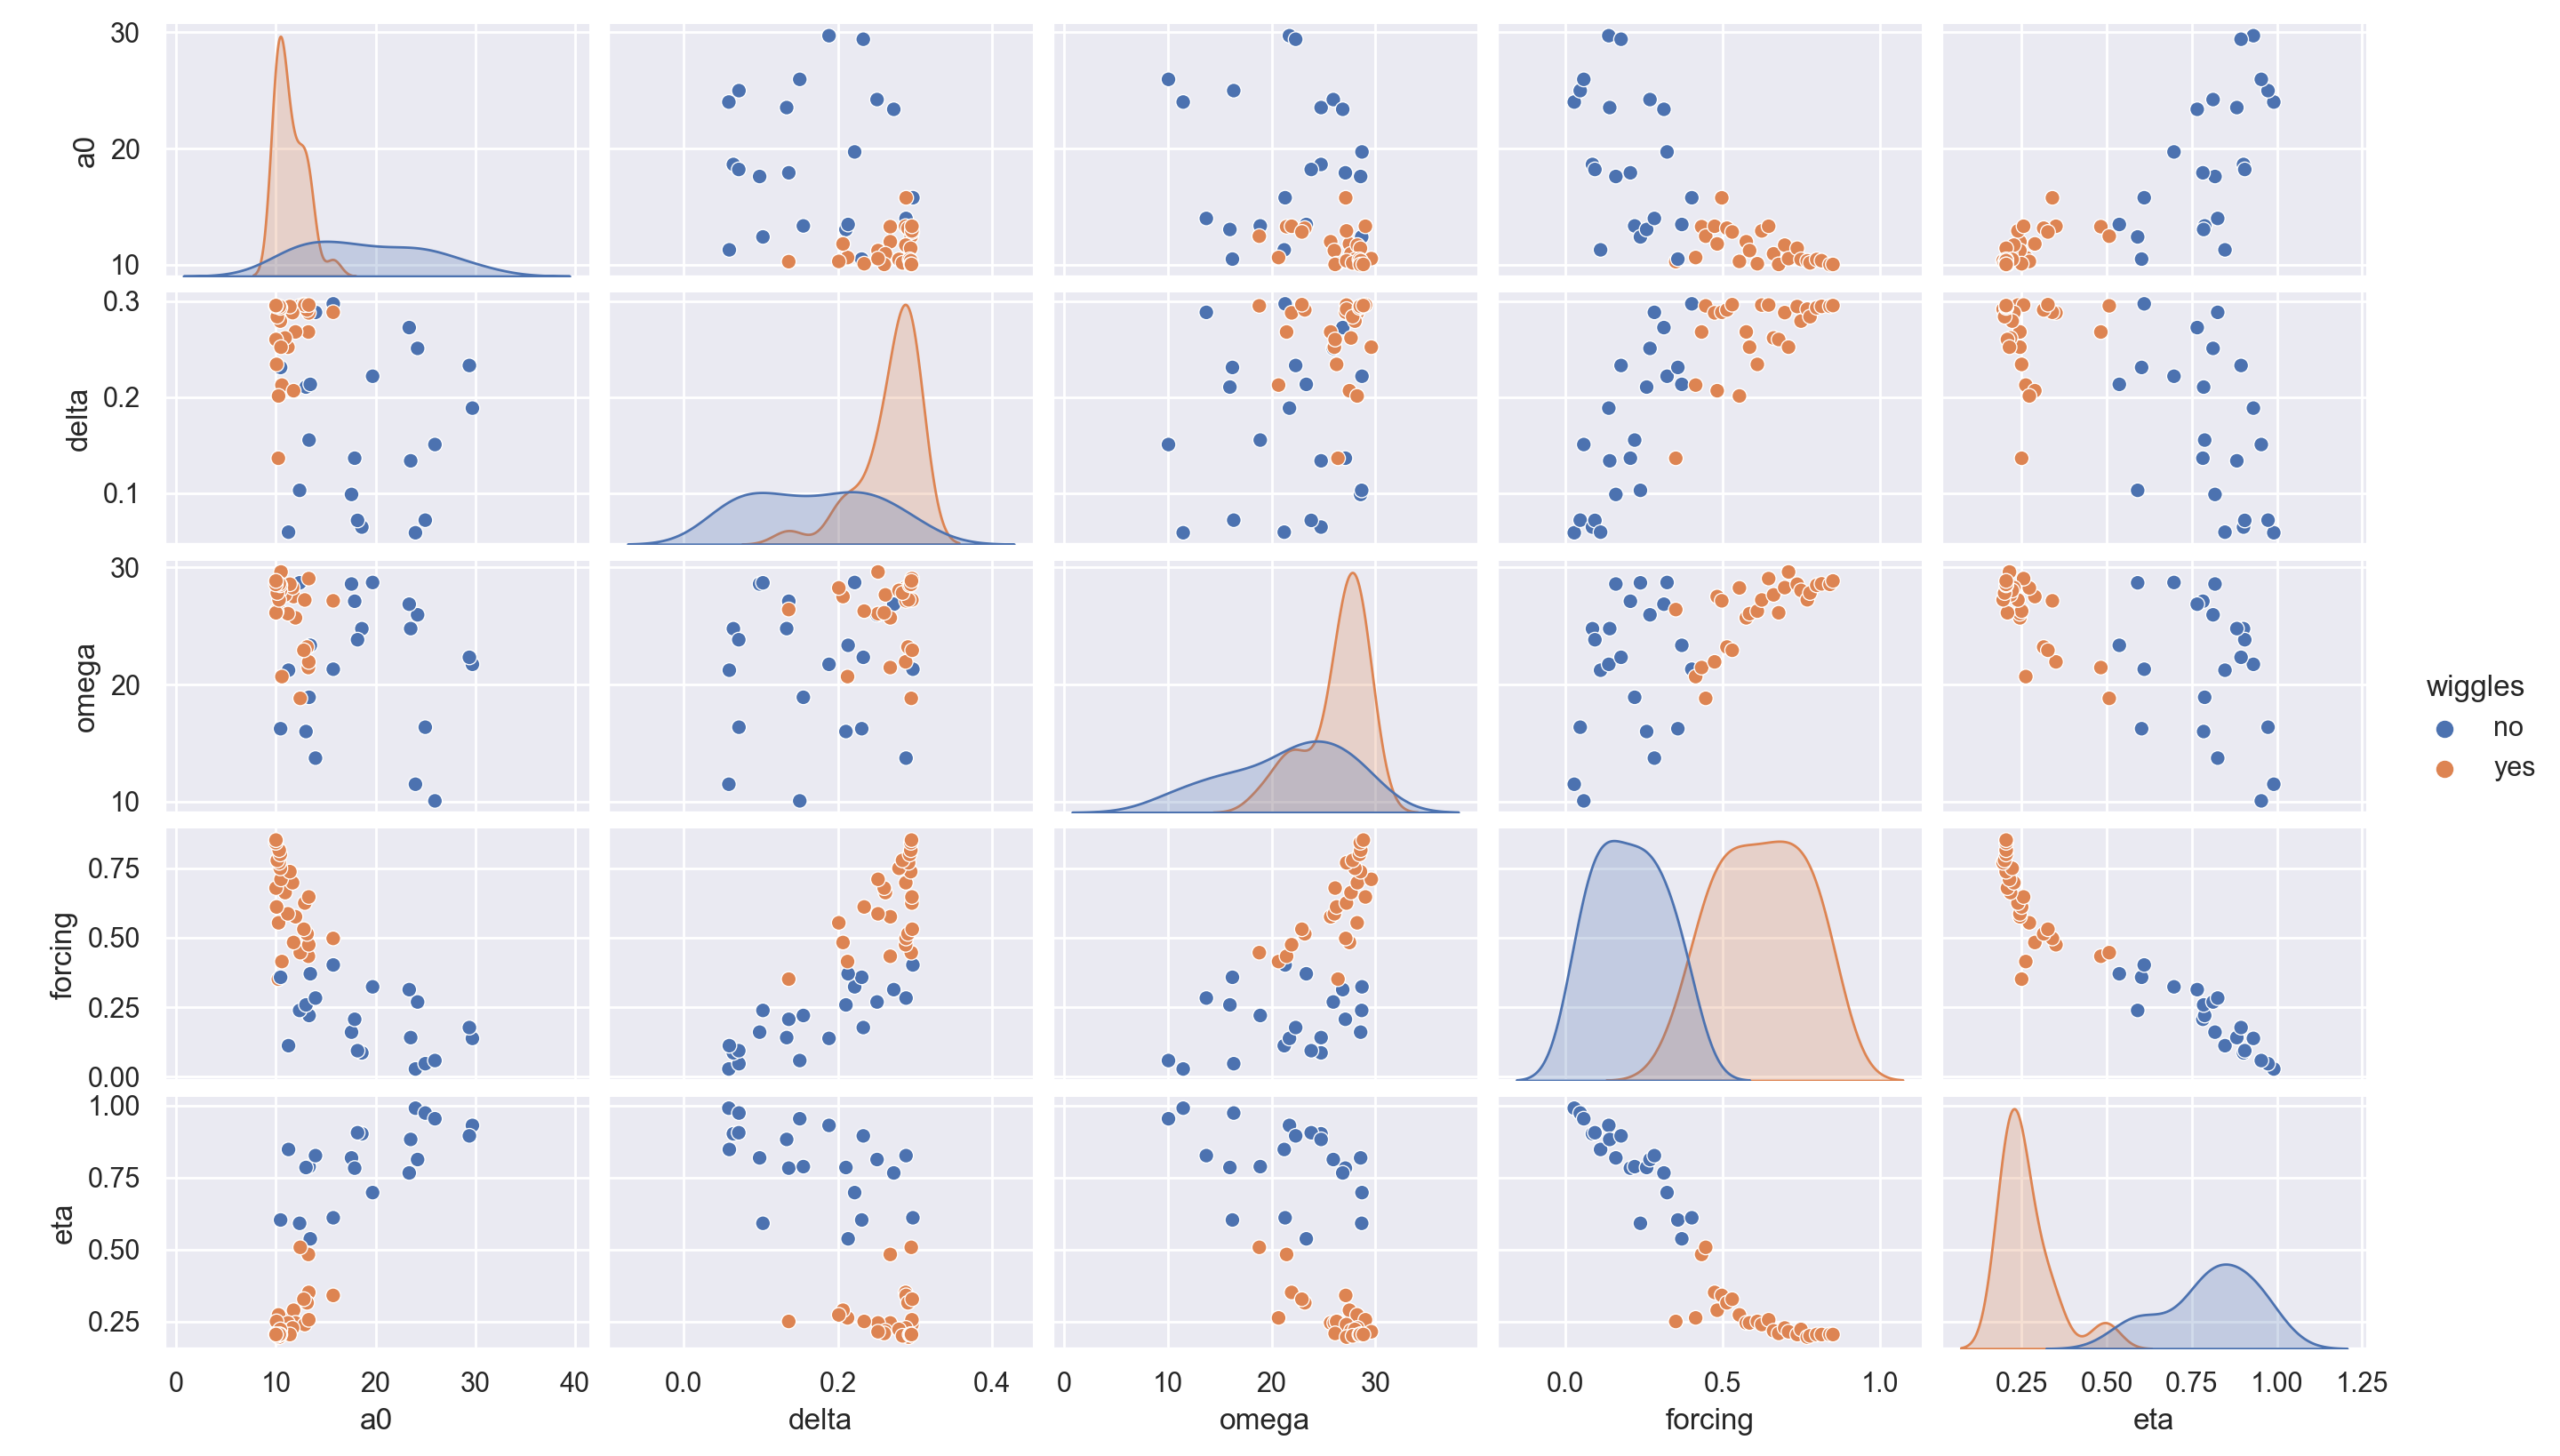
\includegraphics[width=1\columnwidth]{research_project/piston/figures/wiggles/wiggle_correlation.png}
    \caption{Parameter space split by wiggle presence.
    We observe how wiggles are prone to appear for low values in the speed of sound,
    large values in displacement and frequency; that is, when the forcing into the system is larger than a given threshold $u_M$.}
    \label{fig:wiggle_correlation}
\end{figure}
\twocolumn

\end{document}